\documentclass{article}
\usepackage{subcaption}
\usepackage{amsfonts}
\usepackage{amsmath}
\usepackage{amsthm}
\usepackage{algorithm}
\usepackage{algorithmic}
\usepackage{bm}
\usepackage{hyperref}
\usepackage{footmisc}
\usepackage{xcolor}
\DeclareMathOperator\E{\mathbb{E}}
\DeclareMathOperator\Var{\mathrm{Var}}
\def\R{\mathbb{R}}
\def\P{\mathcal{P}}
\usepackage{mathtools}
\DeclarePairedDelimiter\abs{\lvert}{\rvert}
\DeclarePairedDelimiter\norm{\lVert}{\rVert}
\DeclarePairedDelimiter\inner{\langle}{\rangle}
\def\red#1{\textcolor{red}{#1}}
\makeatletter
\newcommand{\algorithmicfunction}{\textbf{function}}
\newcommand{\algorithmicendfunction}{\algorithmicend\ \algorithmicfunction}
\newenvironment{ALC@func}{\begin{ALC@g}}{\end{ALC@g}}
\newcommand{\FUNCTION}[2][default]{\ALC@it\algorithmicfunction\ #2\ %
\textbf{:}%
\ALC@com{#1}\begin{ALC@func}}
\ifthenelse{\boolean{ALC@noend}}{
    \newcommand{\ENDFUNCTION}{\end{ALC@func}}
  }{
    \newcommand{\ENDFUNCTION}{\end{ALC@func}\ALC@it\algorithmicendfunction}
  }
\makeatother
\theoremstyle{definition}
\newtheorem{definition}{Definition}
\newtheorem{theorem}{Theorem}
\newtheorem{example}{Example}
\newtheorem{corollary}{Corollary}
\newtheorem{lemma}{Lemma}
\newtheorem{remark}{Remark}
\title{Paramatric Computing of Info-Clustering}
\begin{document}
\maketitle
Using paramatric maximum flow algorithm to solve the following problem:
\begin{equation}\label{eq:pmq}
\tilde{h}(\lambda) = \min_{j \in A \subseteq V} f(A) - 2\lambda - y^{\lambda}(A)
\end{equation}
where
$y^{\lambda}_i = \min\{a_i - 2\lambda, b_i\}$, where $b_i$ maybe $+\infty$.
The minimum solution to \eqref{eq:pmq} is denoted as $A^{\lambda}$ since different $\lambda$ will produce different set $A$. The structure of the solution is a nested family like \eqref{eq:Alambda}.

If $\lambda$ is sufficiently large, then all $y_i^{\lambda}$ will have the form $a_i - 2 \lambda$ and the minimum solution is $\{j\}$; on the other hand, since we are only concerned about $\lambda \geq 0$. We can compute \eqref{eq:pmq} for $\lambda = -\epsilon$. Then we have $T_0$ and $T_k$ in \eqref{eq:Alambda}.

An important observation of function $\tilde{h}(\lambda)$ is that it is piecewise linear and concave. $T_0$ corresponds a piecewise linear part and $T_k$ corresponds another one.  To compute the nested family between $T_0$ and $T_k$, we use divide and conquer techniques. The algorithm is presented in Algorithm \ref{alg:pmfT}.

\begin{algorithm}
\caption{Theoretical Formulation of Parametric Computing}\label{alg:pmfT}
\begin{algorithmic}[1]
\REQUIRE $y^{\lambda}$ and function $f$
\ENSURE The array \textbf{L} contains $\lambda_1, \dots \lambda_k$. The array $A^{\lambda}$ contains the $T_0,\dots, T_k$. More specificly, $\mathtt{index} = \abs{V} - \abs{T_i}$, $A^{\lambda}[\mathtt{index}]=T_i,  L[\mathtt{index}]=\lambda_{i+1}$\footnotemark
\STATE \textbf{L}, $A^{\lambda} \leftarrow$ empty arrays of size $\abs{V}$
\STATE $Q \leftarrow \argmin_{A\in V} \tilde{h}(-\epsilon), P \leftarrow \{ j \}$
\STATE $A^{\lambda}[ \abs{V}-\abs{Q}]=Q, A^{\lambda}[ \abs{V}-\abs{P}] = P$
\STATE \texttt{Split}$(Q,P)$
\FUNCTION{\texttt{Split}$(Q,P)$}
\STATE Let $\tilde{\lambda}_2$ be the solution to $f(Q) - y^{\lambda}(Q) = f(P) - y^{\lambda}(P)$
\STATE $h' = f(Q) - 2\lambda - y^{\tilde{\lambda}_2}(Q)$
 \STATE $P' =\argmin_{A\in V} \tilde{h}(\tilde{\lambda}_2) $ 
 \IF{$ \tilde{h}(\lambda_2) = h'$}
 	\STATE $\mathbf{L}[\abs{V} - \abs{Q}] = \tilde{\lambda}_2$
 \ELSE
 	\STATE $A^{\lambda}[\abs{V} - \abs{P'}]=P'$
 	\STATE \texttt{Split}$(Q,P')$
 	\STATE \texttt{Split}$(P',P)$
 \ENDIF
\ENDFUNCTION
\end{algorithmic}
\end{algorithm}
\footnotetext{we let $\lambda_{k+1} = +\infty$}

\begin{example}\label{ex:3point}
We consider an example problem. Consider a three node graph (see fig \ref{fig:ex}). $G=(\{1,2,3\},\{(1,2),(1,3),(2,3)| w_{12}=w_{23}=1, w_{13}=5\})$ and $f(A)$ is the graph cut function. Let $j=3$ and $y^{\lambda}_i = -2\lambda$ for $i=1,2,3$.
\begin{figure}[!ht]
\centering
\begin{subfigure}{0.45\textwidth}
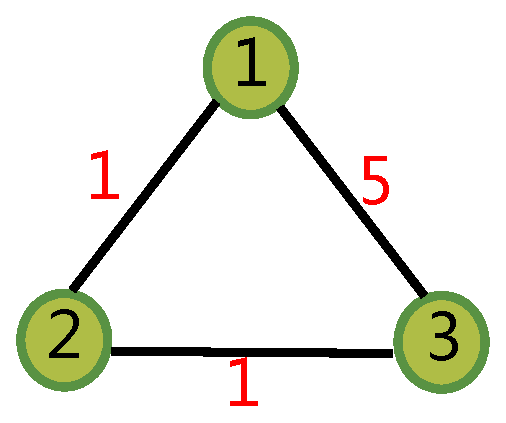
\includegraphics[width=\textwidth]{pic/example.eps}
\caption{A three node graph}\label{fig:ex}
\end{subfigure}
\begin{subfigure}{0.45\textwidth}
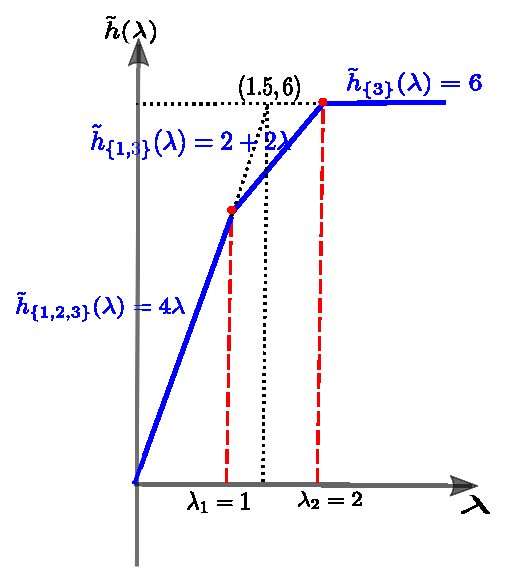
\includegraphics[width=\textwidth]{pic/example_pst.eps}
\caption{method to solve $\tilde{h}(\lambda)$}\label{fig:linseg}
\end{subfigure}
\caption{}
\end{figure}
we can get $T_0 = \{1,2,3\} $ and $T_k = \{3\}$. And their corresponding lines are $4\lambda$ and $6$. As Figure \ref{fig:linseg} shows, they intersect at $(1.5,6)$, the set $T_1=\{1,3\}$; and we can compute $\tilde{h}(1.5)=5<6$. That is, there are turning points at interval $(0, 1.5)$ and $(1.5, +\infty)$ respectively. For the first interval, we compute the intersection of $4\lambda$ and $2+2\lambda$ and get$(1,4)$; Also $\tilde{h}(1)=4$, therefore, the computation for the first interval is finished. The same goes for the second interval. And finally, we can get $L=[\lambda_1, \lambda_2, +\infty]$ and $A^{\lambda} = [\{1,2,3\}, \{1,3\},\{3\}]$
\end{example}

Algorithm \ref{alg:pmfT} is theoretical computable. To make it possible to implenmetation, we need to figure out how to solve $\tilde{\lambda}_2$ and how to compute $\tilde{h}(\lambda)$ for given $\lambda$ efficiently.

To compute $\tilde{h}(\lambda)$ , we need to convert the problem to a weighted directed graph.
For the original graph, each edge is splitted into two directed arc with same capacity.
Introduce a source node $s$ while $j$ is treated as target node.  then change
$c^{\lambda}(s,v)=\max\{0, -y^{\lambda}_v\}, c^{\lambda}(v,j) += \max\{0, y^{\lambda}_v\}$ for $ v=1 $ to $\abs{V}$ and $v \neq  j$.
In detailed form is:
\begin{align}
c(s, v) &=  \max\{0, -\min\{a_i-2\lambda, b_i\}\} \\
c(v, j) & = \tilde{c}(v, j) + \max\{0, \min\{a_i - 2\lambda, b_i\}\}
\end{align}
\begin{figure}
\centering
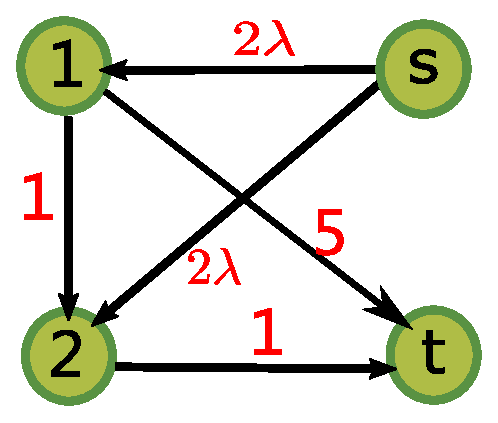
\includegraphics[width=5cm]{pic/example_st.eps}
\caption{converted weighted digraph}\label{fig:convert}
\end{figure}
Figure \ref{fig:convert} illustrates the convertion for Example \ref{ex:3point} and $\lambda>0$ .
Then the minimum minimizer to 
\begin{equation}\label{eq:pmqe}
\min_{s\in U\backslash T, j\in T}c^{\lambda}(U\backslash T, T)
\end{equation}
is the same with equation \eqref{eq:pmq} while the minumum value differs a constant.

Let $\widetilde{G}$ be the modified weighted directed graph from $G$ (add $s$ and modify some capacity). 


By doing so, we can rewrite Algorithm \ref{alg:pmfT} by Algorithm \ref{alg:pmfC}.
\begin{algorithm}
\caption{paramatric maximum flow $(\mathcal{A}, L) = \texttt{pmf}(G(V,E), c(e), j, y^{\lambda})$}\label{alg:pmfC}
\begin{algorithmic}[1]
\REQUIRE an undirected graph $G(V, E)$; $j \in V={1,2,\dots, \abs{V}}$; edge cost function $c(e)$ for $e \in E$; function $f(A)$ is the cut function w.r.t set $A\subseteq V$; tuples $y^{\lambda}_i = (a_i, b_i)$ for $i \in V$.
\ENSURE a nested family of minimal value to equation \eqref{eq:pmq}, as a set list $\mathcal{A}$ and its corresponding turning value $\lambda$ as a value list $L$.
\STATE Let $L$ be the turning point list, initialized as empty array, let $V'=V\cup\{s\}$.
\STATE find $(S_0, T_0)$ which is optimal to \eqref{eq:pmqe} for $ \lambda  = -\epsilon$.  Also let $T_1 = \{j\}$ and $S_1 = \{s\}\cup V \backslash \{j\}$.
\STATE $\mathcal{A}$ contains the decreasing set list, initialized as $[T_0, T_1]$;
\STATE \texttt{slice}$( S_0, T_1)$
\STATE sort $L$ and reverse sort $\mathcal{A}$
\FUNCTION{\texttt{slice}$(S, T)$}
  \STATE Let $\tilde{\lambda}_2$ be the value of $\lambda$ such that $c^{\lambda}(S, V'\backslash S) = 
c^{\lambda}(V'\backslash T, T)$ \label{findLambda}
\STATE for $\lambda = \tilde{\lambda}_2$, find $(S', T')$ which is optimal to \eqref{eq:pmqe} for $\widetilde{G}$.
\IF{$S' \neq S$ and $T' \neq T$}
\STATE insert $T'$ to $\mathcal{A}$
\STATE \texttt{slice}$(S, T')$
\STATE \texttt{slice}$(S', T)$
\ELSE
\STATE insert $\lambda_2$ to $L$
\ENDIF
\ENDFUNCTION
\end{algorithmic}
\end{algorithm}
In Algorithm \ref{alg:pmfC}, the \texttt{slice} function has two parameters:
the first parameter is the subset containing $s$ and the second parameter is the vertice subset containing $j$. It is equivalent to the \texttt{split} function in Algorithm \ref{alg:pmfT}.

When Algorithm \ref{alg:pmfC} terminates, we get $L=[\lambda_1, \lambda_2, \dots, \lambda_{k-1}]$ with
$0 \leq \lambda_1 \footnotemark < \lambda_2 < \dots < \lambda_{k-1}$ and $\mathcal{A} = [T_0, T_1, \dots, T_k]$ with \footnotetext{$\lambda_1 $ can be zero since $I(Z_V)$ can be zero.}
$T_k \subsetneq  \dots \subsetneq T_1 \subsetneq T_0$.  The solution to \eqref{eq:pmq} is then
\begin{equation}\label{eq:Alambda}
\mathcal{A}^{\lambda}=\begin{cases}
T_0 & \lambda < \lambda_1 \\
T_i & \lambda_i \leq \lambda < \lambda_{i+1}, \textrm{ for } i=1, 2, \dots, k-1 \\
T_k & \lambda \geq \lambda_{k}
\end{cases}
\end{equation}
Parametric Representation. For edge cost of the converted directed graph, we have

$\lambda_2$ computing can be simplified in previous. For line \ref{findLambda} in  Algorithm \ref{alg:pmfC},  we can rewrite it as:
\begin{equation*}
\sum_{v\in V'\backslash (S\cup T)} [-y^{\lambda}_v ] = g(T)-g(S\backslash\{s\})
\end{equation*}
where $g(B)$ is the graph cut function of the original graph $G$.

Now we give the algorithm to compute the Dilworth truncation $$\min_{\P}\{f[\P] - \abs{\P} \lambda \}$$for all values of $\lambda$. We call the algorithm parametric Dilworth truncation (Algorithm \ref{alg:pdt}) to distinguish Dilworth truncation algorithm which is applied for a given $\lambda$.
\begin{algorithm}
\caption{paramatric Dilworth truncation $(\P, \mathcal{L})=\texttt{pdt}(G(V,E), c(e))$}\label{alg:pdt}
\begin{algorithmic}[1]
\REQUIRE an undirected graph $G(V, E)$; edge cost function $c(e)$ for $e\in E$
\ENSURE a nested family of partition $\P^{\lambda}$ and its corresponding turning point list $\mathcal{L}$
\STATE initialize $y^{\lambda}_v = (0, +\infty)$ for $ v \in V$, $\P^{\lambda} = [\{\emptyset\}], \mathcal{L} = [+\infty]$
\FOR{$j = 1$ to $\abs{V}$}
\STATE  $(\mathcal{A}, L) = \texttt{pmf}(G(V,E), c(e), j, y^{\lambda})$
\FOR{$u=1$ to $\abs{V}$}
\IF{$u=j$}
\STATE $y^{\lambda}_j = (f(\{j\}), +\infty)$
\ELSE
\STATE $ i = \max_i \{ u \in \mathcal{A}[i]\}$
\IF{$i$ exists and $L[i] > \frac{a_u - b_u}{2}$}
\STATE $y_u^{\lambda} = (a_u, a_u - 2 L[i])$
\ENDIF
\ENDIF
\ENDFOR
\STATE $i, k = 0, \mathcal{Q} = \{\emptyset\}, \widetilde{\mathcal{\P}}^{\lambda} = [], \widetilde{\mathcal{L}} = []$, append $+\infty$ to $L$.
\WHILE{$i<\texttt{length}(\mathcal{L})$ \texttt{ and } $k<\texttt{length}(L)$}
\IF{$ \P^{\lambda}_i[\mathcal{A}_k] \neq \mathcal{Q}$}
\STATE $\mathcal{Q} = \P^{\lambda}_i[\mathcal{A}_k]$
\STATE append $\mathcal{Q}$ to $\widetilde{\mathcal{\P}}^{\lambda}$ and $\min\{\mathcal{L}[i], L[k]\}$
to $\widetilde{\mathcal{L}}$
\ELSE
\STATE $\widetilde{\mathcal{L}}[-1] = \min\{\mathcal{L}[i], L[k]\}$
\ENDIF
\STATE $(i, k) \leftarrow \begin{cases} (i+1, k) & \mathcal{L}[i] < L[k] \\  (i, k+1) & \mathcal{L}[i] > L[k]\\ (i+1, k+1) & \mathcal{L}[i] = L[k]\end{cases}$
\ENDWHILE
\STATE $(\P^{\lambda}, \mathcal{L}) \leftarrow (\widetilde{\mathcal{\P}}^{\lambda},  \widetilde{\mathcal{L}})$
\ENDFOR
\end{algorithmic}
\end{algorithm}
\end{document}
